\section{IL DASM}
\subsection{exe only}
\begin{figure}[htbp]
	\centering
	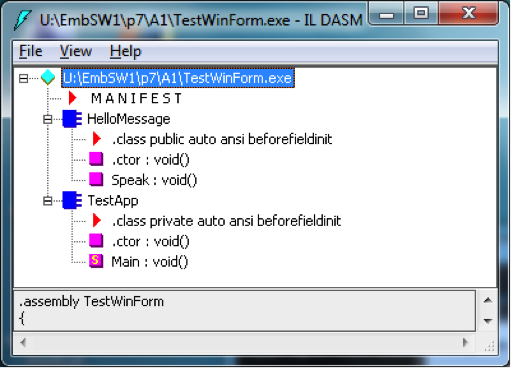
\includegraphics[width=7cm]{images/ILDASM_exe.png}
\end{figure}

\subsubsection{Manifest}
\begin{lstlisting}[style=Csharp]
// Metadata version: v4.0.30319
.assembly extern mscorlib
{
  .publickeytoken = (B7 7A 5C 56 19 34 E0 89 )                         // .z\V.4..
  .ver 4:0:0:0
}
.assembly extern System.Windows.Forms
{
  .publickeytoken = (B7 7A 5C 56 19 34 E0 89 )                         // .z\V.4..
  .ver 4:0:0:0
}
.assembly TestWinForm
{
  .custom instance void [mscorlib]System.Runtime.CompilerServices.CompilationRelaxationsAttribute::.ctor(int32) = ( 01 00 08 00 00 00 00 00 ) 
  .custom instance void [mscorlib]System.Runtime.CompilerServices.RuntimeCompatibilityAttribute::.ctor() = ( 01 00 01 00 54 02 16 57 72 61 70 4E 6F 6E 45 78   // ....T..WrapNonEx
  63 65 70 74 69 6F 6E 54 68 72 6F 77 73 01 )       // ceptionThrows.
  .hash algorithm 0x00008004
  .ver 0:0:0:0
}
.module TestWinForm.exe
// MVID: {1C2FC52F-C538-4AE1-B2C5-0653423AC3FD}
.imagebase 0x00400000
.file alignment 0x00000200
.stackreserve 0x00100000
.subsystem 0x0003       // WINDOWS_CUI
.corflags 0x00000001    //  ILONLY
// Image base: 0x0000000001FF0000
\end{lstlisting}

\subsubsection{HelloMessage}
\textbf{.class public auto ansi beforefieldinit}
\begin{lstlisting}[style=Csharp]
.class public auto ansi beforefieldinit HelloMessage
       extends [mscorlib]System.Object
{
} // end of class HelloMessage
\end{lstlisting}

\textbf{.ctor : void()}
\begin{lstlisting}[style=Csharp]
.method public hidebysig specialname rtspecialname 
        instance void  .ctor() cil managed
{
  // Code size       7 (0x7)
  .maxstack  8
  IL_0000:  ldarg.0
  IL_0001:  call       instance void [mscorlib]System.Object::.ctor()
  IL_0006:  ret
} // end of method HelloMessage::.ctor
\end{lstlisting}

\textbf{Speak : void()}
\begin{lstlisting}[style=Csharp]
.method public hidebysig instance void  Speak() cil managed
{
  // Code size       13 (0xd)
  .maxstack  8
  IL_0000:  nop
  IL_0001:  ldstr      "Hello..."
  IL_0006:  call       valuetype [System.Windows.Forms]System.Windows.Forms.DialogResult [System.Windows.Forms]System.Windows.Forms.MessageBox::Show(string)
  IL_000b:  pop
  IL_000c:  ret
} // end of method HelloMessage::Speak
\end{lstlisting}


\subsection{dll + exe}
\subsubsection{DLL}
\begin{figure}[htbp]
	\centering
	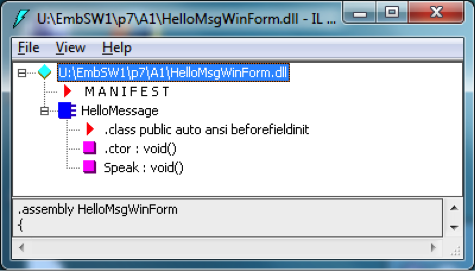
\includegraphics[width=7cm]{images/ILDASM_dll_dll.png}
\end{figure}

\textbf{Manifest}
\begin{lstlisting}[style=Csharp]
// Metadata version: v4.0.30319
.assembly extern mscorlib
{
  .publickeytoken = (B7 7A 5C 56 19 34 E0 89 )                         // .z\V.4..
  .ver 4:0:0:0
}
.assembly extern System.Windows.Forms
{
  .publickeytoken = (B7 7A 5C 56 19 34 E0 89 )                         // .z\V.4..
  .ver 4:0:0:0
}
.assembly HelloMsgWinForm
{
  .custom instance void [mscorlib]System.Runtime.CompilerServices.CompilationRelaxationsAttribute::.ctor(int32) = ( 01 00 08 00 00 00 00 00 ) 
  .custom instance void [mscorlib]System.Runtime.CompilerServices.RuntimeCompatibilityAttribute::.ctor() = ( 01 00 01 00 54 02 16 57 72 61 70 4E 6F 6E 45 78   // ....T..WrapNonEx
  63 65 70 74 69 6F 6E 54 68 72 6F 77 73 01 )       // ceptionThrows.
  .hash algorithm 0x00008004
  .ver 0:0:0:0
}
.module HelloMsgWinForm.dll
// MVID: {234AA45E-1346-4FB2-B682-0EBE788AE35C}
.imagebase 0x10000000
.file alignment 0x00000200
.stackreserve 0x00100000
.subsystem 0x0003       // WINDOWS_CUI
.corflags 0x00000001    //  ILONLY
// Image base: 0x0000000000750000
\end{lstlisting}

\textbf{.class public auto ansi beforefieldinit}
\begin{lstlisting}[style=Csharp]
.class public auto ansi beforefieldinit HelloMessage
       extends [mscorlib]System.Object
{
} // end of class HelloMessage
\end{lstlisting}

\textbf{.ctor : void()}
\begin{lstlisting}[style=Csharp]
.method public hidebysig specialname rtspecialname 
        instance void  .ctor() cil managed
{
  // Code size       7 (0x7)
  .maxstack  8
  IL_0000:  ldarg.0
  IL_0001:  call       instance void [mscorlib]System.Object::.ctor()
  IL_0006:  ret
} // end of method HelloMessage::.ctor
\end{lstlisting}

\textbf{Speak : void()}
\begin{lstlisting}[style=Csharp]
.method public hidebysig instance void  Speak() cil managed
{
  // Code size       13 (0xd)
  .maxstack  8
  IL_0000:  nop
  IL_0001:  ldstr      "Hello..."
  IL_0006:  call       valuetype [System.Windows.Forms]System.Windows.Forms.DialogResult [System.Windows.Forms]System.Windows.Forms.MessageBox::Show(string)
  IL_000b:  pop
  IL_000c:  ret
} // end of method HelloMessage::Speak
\end{lstlisting}

\subsubsection{TestApp}
\textbf{.class private auto ansi beforefieldinit}
\begin{lstlisting}[style=Csharp]
.class private auto ansi beforefieldinit TestApp
       extends [mscorlib]System.Object
{
} // end of class TestApp
\end{lstlisting}

\textbf{.ctor : void()}
\begin{lstlisting}[style=Csharp]
.method public hidebysig specialname rtspecialname 
        instance void  .ctor() cil managed
{
  // Code size       7 (0x7)
  .maxstack  8
  IL_0000:  ldarg.0
  IL_0001:  call       instance void [mscorlib]System.Object::.ctor()
  IL_0006:  ret
} // end of method TestApp::.ctor
\end{lstlisting}

\textbf{Main : void()}
\begin{lstlisting}[style=Csharp]
.method public hidebysig static void  Main() cil managed
{
  .entrypoint
  // Code size       15 (0xf)
  .maxstack  1
  .locals init (class HelloMessage V_0)
  IL_0000:  nop
  IL_0001:  newobj     instance void HelloMessage::.ctor()
  IL_0006:  stloc.0
  IL_0007:  ldloc.0
  IL_0008:  callvirt   instance void HelloMessage::Speak()
  IL_000d:  nop
  IL_000e:  ret
} // end of method TestApp::Main
\end{lstlisting}


\subsection{EXE}
\begin{figure}[htbp]
	\centering
	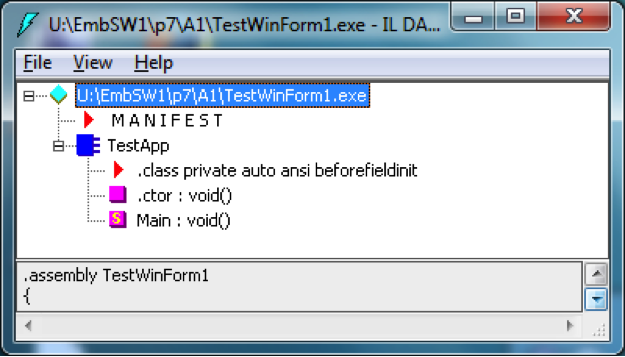
\includegraphics[width=7cm]{images/ILDASM_dll_exe.png}
\end{figure}

\textbf{Manifest}
\begin{lstlisting}[style=Csharp]
// Metadata version: v4.0.30319
.assembly extern mscorlib
{
  .publickeytoken = (B7 7A 5C 56 19 34 E0 89 )                         // .z\V.4..
  .ver 4:0:0:0
}
.assembly extern HelloMsgWinForm
{
  .ver 0:0:0:0
}
.assembly TestWinForm1
{
  .custom instance void [mscorlib]System.Runtime.CompilerServices.CompilationRelaxationsAttribute::.ctor(int32) = ( 01 00 08 00 00 00 00 00 ) 
  .custom instance void [mscorlib]System.Runtime.CompilerServices.RuntimeCompatibilityAttribute::.ctor() = ( 01 00 01 00 54 02 16 57 72 61 70 4E 6F 6E 45 78   // ....T..WrapNonEx
  63 65 70 74 69 6F 6E 54 68 72 6F 77 73 01 )       // ceptionThrows.
  .hash algorithm 0x00008004
  .ver 0:0:0:0
}
.module TestWinForm1.exe
// MVID: {7FA99F0B-33EB-4BD0-977B-54AAC8599C6F}
.imagebase 0x00400000
.file alignment 0x00000200
.stackreserve 0x00100000
.subsystem 0x0003       // WINDOWS_CUI
.corflags 0x00000001    //  ILONLY
// Image base: 0x0000000000750000
\end{lstlisting}

\textbf{.class private auto ansi beforefieldinit}
\begin{lstlisting}[style=Csharp]
.class private auto ansi beforefieldinit TestApp
       extends [mscorlib]System.Object
{
} // end of class TestApp
\end{lstlisting}

\textbf{.ctor : void()}
\begin{lstlisting}[style=Csharp]
.method public hidebysig specialname rtspecialname 
        instance void  .ctor() cil managed
{
  // Code size       7 (0x7)
  .maxstack  8
  IL_0000:  ldarg.0
  IL_0001:  call       instance void [mscorlib]System.Object::.ctor()
  IL_0006:  ret
} // end of method TestApp::.ctor
\end{lstlisting}

\textbf{Main : void()}
\begin{lstlisting}[style=Csharp]
.method public hidebysig static void  Main() cil managed
{
  .entrypoint
  // Code size       15 (0xf)
  .maxstack  1
  .locals init (class [HelloMsgWinForm]HelloMessage V_0)
  IL_0000:  nop
  IL_0001:  newobj     instance void [HelloMsgWinForm]HelloMessage::.ctor()
  IL_0006:  stloc.0
  IL_0007:  ldloc.0
  IL_0008:  callvirt   instance void [HelloMsgWinForm]HelloMessage::Speak()
  IL_000d:  nop
  IL_000e:  ret
} // end of method TestApp::Main
\end{lstlisting}